%! suppress = MissingImport
%! suppress = MissingLabel
%! suppress = LineBreak

% CLI args https://tex.stackexchange.com/a/1501
\newif\ifhandout
\input{flags}

%! suppress = MissingLabel
%! suppress = DocumentclassNotInRoot
%! suppress = DiscouragedUseOfDef

% * Make friends tikz & colors
%   https://en.wikibooks.org/wiki/LaTeX/Colors
% * To enable vertical top alignment globally
%   https://tex.stackexchange.com/questions/9889/positioning-content-at-the-top-of-a-beamer-slide-by-default
% * Set handout from CLI
%   https://tex.stackexchange.com/a/1501
\ifhandout
\documentclass[usenames, dvipsnames, handout]{beamer} % https://tex.stackexchange.com/questions/224091/beamer-how-to-disable-pause-temporarily
\else
\documentclass[usenames, dvipsnames]{beamer}
\fi
% ------------------------------------------------

% Graphics
\usepackage{color}
\usepackage{tabularx}
\usepackage{tikz}
% https://tikz.dev/tikz-graphs
\usetikzlibrary{positioning, shapes.geometric, arrows, automata, graphs}
\tikzset{
    expr/.style={ellipse, draw=gray!60, fill=gray!5, very thick, minimum size=7mm, yshift=0.7cm},
    hexpr/.style={ellipse, draw=gray!60, fill=blue!15, very thick, minimum size=7mm, yshift=0.7cm},
    stmt/.style={rectangle, draw=gray!60, fill=gray!5, very thick, minimum size=5mm, yshift=0.7cm},
    decl/.style={rectangle, draw=blue!60, fill=gray!5, very thick, minimum size=5mm, yshift=0.7cm},
    hdecl/.style={rectangle, draw=blue!60, fill=blue!15, very thick, minimum size=5mm, yshift=0.7cm},
    subtree/.style={shape border rotate=90, isosceles triangle, draw=gray!60, fill=gray!5, very thick, minimum size=5mm, yshift=0.0cm},
}
\usepackage{blkarray}
\usepackage{graphicx}
\usepackage{forest} % https://tex.stackexchange.com/questions/198405/how-to-change-the-color-of-subtrees-in-tikz-qtree
% ------------------------------------------------

% Math
\usepackage{amsmath, amsfonts}
\usepackage{amssymb}
\usepackage{proof}
\usepackage{mathrsfs}
% Crossed-out symbols
% https://tex.stackexchange.com/questions/75525/how-to-write-crossed-out-math-in-latex
\usepackage[makeroom]{cancel}
\usepackage{mathtools}
% ------------------------------------------------

% Additional font sizes
% https://www.overleaf.com/learn/latex/Questions/How_do_I_adjust_the_font_size%3F
\usepackage{moresize}
% Additional colors
% https://www.overleaf.com/learn/latex/Using_colours_in_LaTeX
\usepackage{xcolor}
% Textual math symbols
\usepackage{textcomp}
% ------------------------------------------------

% Language
\usepackage[utf8] {inputenc}
\usepackage[T2A] {fontenc}
\usepackage[english, russian] {babel}
\usepackage{indentfirst, verbatim}
\usetikzlibrary{cd, babel}
% ------------------------------------------------

% Fonts: https://sites.math.washington.edu/~reu/docs/latex_symbols.pdf
\usepackage{stmaryrd}
\usepackage{cmbright}
\usepackage{wasysym}
\usepackage[weather]{ifsym} % https://tex.stackexchange.com/questions/100424/how-to-use-the-ifsym-package
% https://tex.stackexchange.com/questions/615300/pdflatex-builtin-glyph-names-is-empty
\pdfmapline{=dictsym DictSym <dictsym.pfb}
\pdfmapline{=pigpen <pigpen.pfa}
\usepackage{dictsym}
% ------------------------------------------------

% Code
% * Needs -shell-escape build flag
%   https://tex.stackexchange.com/questions/99475/how-to-invoke-latex-with-the-shell-escape-flag-in-texstudio-former-texmakerx
% * Set build directory
%   https://tex.stackexchange.com/questions/339931/latex-minted-package-using-custom-output-directory-build
\usepackage{minted}
\setminted{xleftmargin=\parindent, autogobble, escapeinside=\#\#}
% ------------------------------------------------

% Template
\usetheme{CambridgeUS}
\usecolortheme{dolphin}
% https://tex.stackexchange.com/questions/231439/beamer-how-to-make-font-larger-for-page-numbers
\setbeamerfont{headline}{size=\scriptsize}
\setbeamerfont{footline}{size=\scriptsize}
% Remove heddline
% https://tex.stackexchange.com/questions/33146/how-could-i-remove-a-header-in-a-beamer-presentation
%\setbeamertemplate{headline}{}
% Slide sizes
% https://tex.stackexchange.com/questions/56768/how-to-set-a-small-default-font-size-with-beamer
%\geometry{paperwidth=140mm,paperheight=105mm} % 4:3
\geometry{paperwidth=168mm,paperheight=105mm} % 16:10
% Remove navigation bar
% https://stackoverflow.com/questions/3210205/how-to-get-rid-of-navigation-bars-in-beamer
\beamertemplatenavigationsymbolsempty
% ------------------------------------------------

% Bullets
% https://9to5science.com/change-bullet-style-formatting-in-beamer
% https://tex.stackexchange.com/questions/185742/i-need-to-change-color-of-beamer-itemize-and-subitem-separately
\setbeamertemplate{itemize item}{\scriptsize\raise1.25pt\hbox{\donotcoloroutermaths$\blacktriangleright$}}
\setbeamertemplate{itemize subitem}{\scriptsize\raise1.5pt\hbox{\donotcoloroutermaths$\blacktriangleright$}}
\setbeamertemplate{itemize subsubitem}{\tiny\raise1.5pt\hbox{\donotcoloroutermaths$\blacktriangleright$}}
\setbeamertemplate{enumerate item}{\insertenumlabel.}
\setbeamertemplate{enumerate subitem}{\insertenumlabel.\insertsubenumlabel}
\setbeamertemplate{enumerate subsubitem}{\insertenumlabel.\insertsubenumlabel.\insertsubsubenumlabel}
% ------------------------------------------------

% Table of contents format
% https://tex.stackexchange.com/questions/642927/format-table-of-contents-in-beamer
\setbeamertemplate{section in toc}{%
        {\color{blue}\inserttocsectionnumber.}
    \inserttocsection\par%
}
\setbeamertemplate{subsection in toc}{%
        {\color{blue}\hspace{1em}\scriptsize\raise1.25pt\hbox{\donotcoloroutermaths$\blacktriangleright$}}
    \inserttocsubsection\par%
}
\setbeamertemplate{subsubsection in toc}{%
        {\color{blue}\hspace{2em}\tiny\raise1.25pt\hbox{\donotcoloroutermaths$\blacktriangleright$}}
    \inserttocsubsubsection\par%
}
% ------------------------------------------------

% Misc
\usepackage{multicol}
\usepackage{hyperref}
\usepackage{soul} % https://tex.stackexchange.com/questions/23711/strikethrough-text
% ------------------------------------------------

% Fix \pause for amsmath package envs (black black magic)
% https://tex.stackexchange.com/questions/16186/equation-numbering-problems-in-amsmath-environments-with-pause/75550#75550
% https://tex.stackexchange.com/questions/6348/problem-with-beamers-pause-in-alignments
%! suppress = Makeatletter
\makeatletter
\let\save@measuring@true\measuring@true
\def\measuring@true{%
    \save@measuring@true
    \def\beamer@sortzero##1{\beamer@ifnextcharospec{\beamer@sortzeroread{##1}}{}}%
    \def\beamer@sortzeroread##1<##2>{}%
    \def\beamer@finalnospec{}%
}
%! suppress = Makeatletter
\makeatother
% ------------------------------------------------

% Sections
\newcommand{\sectionplan}[1]{\section{#1}%
    \begin{frame}[noframenumbering]{Содержание}
        \tableofcontents[currentsection]
    \end{frame}
}
\newcommand{\subsectionplan}[1]{\subsection{#1}%
    \begin{frame}[noframenumbering]{Содержание}
        \tableofcontents[currentsubsection]
    \end{frame}
}
% ------------------------------------------------

% Footnotes
\renewcommand{\thefootnote}{\arabic{footnote}}
\renewcommand{\thempfootnote}{\arabic{mpfootnote}}
% https://tex.stackexchange.com/questions/28465/multiple-footnotes-at-one-point
\usepackage{fnpct}
% ------------------------------------------------

% Links
% Colors also links on slide foot.
%\hypersetup{
%    colorlinks=true,
%    citecolor=blue,
%    linkcolor=blue,
%    urlcolor=blue
%}
% ------------------------------------------------

% Appendix
% Slide numbers
% https://tex.stackexchange.com/questions/70448/dont-count-backup-slides
\usepackage{appendixnumberbeamer}
\newcommand{\backupbegin}{
    \newcounter{framenumbervorappendix}
    \setcounter{framenumbervorappendix}{\value{framenumber}}
}
\newcommand{\backupend}{
    \addtocounter{framenumbervorappendix}{-\value{framenumber}}
    \addtocounter{framenumber}{\value{framenumbervorappendix}}
}
% ------------------------------------------------

% Custom commands
% * Decor
\newcommand{\newtopic}[0]{$+$} % item: new topic on "in previous series"
\newcommand{\then}{$\Rightarrow$} % item: consequences
\newcommand{\pop}[0]{\SunCloud} %item:  general eduation
\newcommand{\popslide}[0]{(\pop)}
\newcommand{\advanced}[0]{$\varhexstar$} % item: advanced science
\newcommand{\advancedslide}[0]{(\advanced)}
\newcommand{\practical}[0]{\dstechnical} % item: practical programming notions
\newcommand{\practicalslide}[0]{(\practical)}
\newcommand{\todo}[0]{todo} % item: question
\newcommand{\answer}[0]{\Lightning} % item: answer to the previous question
\newcommand{\eg}[0]{e.g.} % item: example
\newcommand{\defi}[0]{$\Delta$} % item: definition on smth
\newcommand{\textdefi}[1]{\textbf{#1}}
\newcommand{\positive}{$+$} % item: pros
\newcommand{\negative}{{\color{red} $-$}} % item: cons
\newcommand%! suppress = EscapeHashOutsideCommand
\NB[1][0.3]{N\kern-#1em{B}} % default kern amount: -0.3em
\renewcommand{\emph}[1]{{\color{blue} \textit{#1}}}
\newcommand{\vocab}[1]{\textbf{#1}} % item: important new word
% * Lambda calculi
\newcommand{\comb}[1]{\mathbf{#1}} % defined combinator
\newcommand{\term}[1]{\mathbf{#1}} % predefined lambda-term reference
\newcommand{\termdef}{\coloneqq} % lamda term binding
\newcommand{\step}{\rightsquigarrow} % reduction step
\newcommand{\sstep}{\twoheadrightarrow} % multiple steps reduction
\newcommand{\ap}{~} % lambda-term application
\newcommand{\subst}[3]{\left[#2 \mapsto #3 \right] #1} % substitution
\newcommand{\eqbeta}{=_\beta} % beta equality
\newcommand{\eqeta}{=_\eta} % eta-equality
\newcommand{\eqt}{=} % tree-equality of terms
\newcommand{\tlist}[1]{\term{[}#1\term{]}} % list-term
% * Legacy
%\newcommand{\err}[0]{\textcolor{red}{ошибка}} % compilation error

% ------------------------------------------------

% Speaker notes
% https://tex.stackexchange.com/questions/114219/add-notes-to-latex-beamer
% https://tex.stackexchange.com/questions/35444/split-beamer-notes-across-multiple-notes-pages/35496#35496
%\setbeameroption{show notes on second screen=right} % enable speaker notes
%--------------------------------------

\author[]{Андрей Стоян, Илья Колегов, Дмитрий Халанский}
\institute[MSE ITMO]{MSE ITMO}

\setminted{xleftmargin=\parindent, autogobble, escapeinside=??}
\newcommand{\iso}{\sim}

\title{5. Интерпретаторы}
\author{Андрей Стоян}
\institute[ИПКН ИТМО]{ИПКН ИТМО}

\date{осень 2025}

\begin{document}

    \mymaketitle

    \begin{frame}[noframenumbering]{Содержание}
        \tableofcontents
    \end{frame}

    \sectionplan{Башня интерпретаторов}

    \begin{frame}[fragile]{Башня интерпретаторов}
        \pause
        \[U_M^N : N\times D\to D\]
        \pause
        \[d_{out} = U_M^N\left( \underbrace{\langle p_N, d_{in} \rangle}_{\in N\times D} \right)\]
        \pause
        \[
            d_{out} = U^{x86}\left(\left<\underbrace{U_{x86}^{Asm}}_{\in x86}, \underbrace{\overbrace{\langle p_{Asm}}^{\in Asm}, \overbrace{d_{in} \rangle}^{\in D}}_{\in D} \right>\right)
        \]
        \pause
        \[
            d_{out} =
            U^{x86}\left(\left<
                             U_{x86}^{Asm}, \left<
                                                U^C_{Asm}, \left<
                                                               U^{Has}_C, \left< p_{Has}, d_{in}
                        \right>\right>\right>\right>\right)
        \]
    \end{frame}

    \begin{frame}[fragile]{Интерпретаторы повсюду}
        \pause
        \begin{minted}{haskell}
            eval :: Expr -> Int
            eval prog = case prog of
              Const x -> x
              Plus l r -> eval l + eval r
        \end{minted}
    \end{frame}

    \begin{frame}[fragile]{Денотационная семантика}
        \pause
        \[
            \sembr{\bullet} : L \mapsto D
        \]
        \pause
        \[
            \begin{array}{lcl}
                \sembr{n}     & = & 1                            \\
                \sembr{l + r} & = & 1 + \max{(\sembr{l}, \sembr{r})}
            \end{array}
        \]
        \pause
        \[
            \begin{array}{lcl}
                \sembr{n}     & = & n                     \\
                \sembr{l + r} & = & \sembr{l} + \sembr{r}
            \end{array}
        \]
        \pause
        \[
            \begin{array}{lcl}
                \sembr{n}(m)     & = & n                           \\
                \sembr{l + r}(m) & = & \sembr{l}(m) + \sembr{r}(m) \\
                \sembr{input}(m) & = & m
            \end{array}
        \]
    \end{frame}

    \begin{frame}[fragile]{Денотационная семантика на Haskell}
        \pause
        \[
            \begin{array}{lcl}
                \sembr{n}(m)     & = & n                           \\
                \sembr{l + r}(m) & = & \sembr{l}(m) + \sembr{r}(m) \\
                \sembr{input}(m) & = & m
            \end{array}
        \]
        \pause
        \begin{minted}{haskell}
            eval :: Prog -> (Nat -> Nat)
            eval = \case
              Val n -> \_ -> n
              Plus l r -> \m -> eval l m + eval r m
              Input -> \m -> m
        \end{minted}
    \end{frame}

    \begin{frame}[fragile]{Смысл конструкций задаётся как операции над доменом}
        \begin{figure}[h]
            \centering
            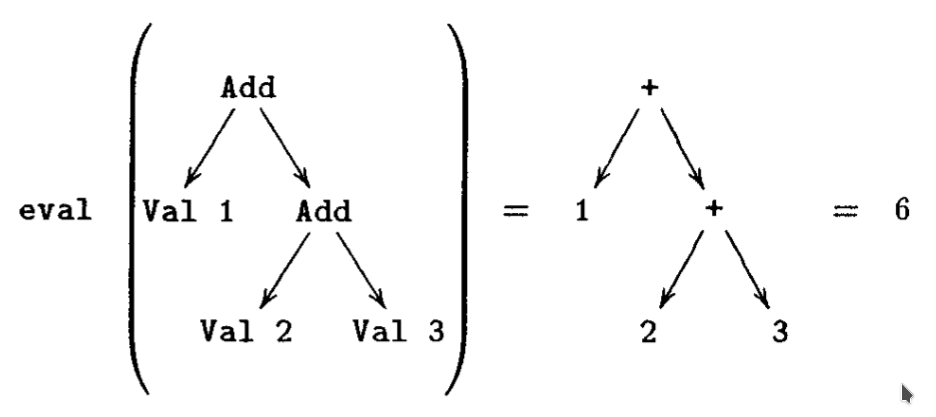
\includegraphics[width=0.6\textwidth]{figs/eval-prog}
        \end{figure}
    \end{frame}

    \begin{frame}[fragile]{Встроенные доменно-специфичные языки}
        \pause
        Deep eDSL:
        \begin{minted}{haskell}
            f :: Int -> Int
            f = eval $ Const 1 `Plus` Input
        \end{minted}
        \pause\vspace{1em}
        Shallow eDSL:
        \begin{minted}{haskell}
            cnst :: Int -> (Int -> Int)
            cnst x _ = x

            input :: Int -> Int
            input env = env

            plus :: (Int -> Int) -> (Int -> Int) -> (Int -> Int)
            plus l r env = l env + r env

            f :: Int -> Int
            f = cnst 1 `plus` input
        \end{minted}
    \end{frame}

    \begin{frame}[fragile]{Meta-circular интерпретаторы}
        \pause
        \begin{minted}{haskell}
            interpret term = case term of
              App f t -> (interpret f) (interpret t)
              If c t e -> if interpret c then interpret t else interpret e
              ...
        \end{minted}
    \end{frame}

    \begin{frame}[fragile]{Пример: библиотека Accelerate}
        \pause
        \begin{minted}{haskell}
            example :: Acc (Vector Int) -> Acc (Vector Int) -> Acc (Vector Int)
            example xs ys = A.zipWith (+) xs ys
        \end{minted}
    \end{frame}

    \sectionplan{Типы значений}

    \begin{frame}[fragile]{Untyped tagless interpreters}
        \pause
        \begin{minted}{haskell}
            data Expr = Const Int | IsZero Expr | If Expr Expr Expr

            evalUnsafe :: Expr -> forall res . res
            evalUnsafe = \case
              Const val -> unsafeCoerce val
              IsZero cond -> unsafeCoerce $ evalUnsafe @Int cond == 0
              If c t e -> if evalUnsafe c then evalUnsafe t else evalUnsafe e
        \end{minted}
    \end{frame}

    \begin{frame}[fragile]{Typed tagged interpreters}
        \pause
        \begin{minted}{haskell}
            data Expr = Const Int | IsZero Expr | If Expr Expr Expr

            data RtValue = RtBool Bool | RtInt Int

            evalRt :: Expr -> RtValue
            evalRt (IsZero expr) = case evalRt expr of
              RtBool value -> error "Type error"
              RtInt value -> RtBool (value == 0)
            -- ...
        \end{minted}
    \end{frame}

    \begin{frame}[fragile]{Typed tagless interpreters}
        \pause
        \begin{equation*}{}
            \infer[Const]{Const~n : int}{n : Int}
            \quad
            \infer[IsZero]{IsZero~n : bool}{n : int}
            \quad
            \infer[If]{If~c~t~e : \tau}{c : bool & t : \tau & e : \tau}
        \end{equation*}
        \pause
        \begin{minted}{haskell}
            data Expr ty where
              Const :: Int -> Expr Int
              IsZero :: Expr Int -> Expr Bool
              If :: forall ty . Expr Bool -> Expr ty -> Expr ty -> Expr ty

            eval :: Expr ty -> ty
            eval = \case
              Const n -> n
              IsZero e -> eval e == 0
              If c t e -> if eval c then eval t else eval e
        \end{minted}
    \end{frame}

    \sectionplan{Связывания и функции первого класса}

    \begin{frame}[fragile]{Let-in через функции}
        \pause
        \[
            \term{let} \ap x \termdef N \ap \term{in} \ap M \equiv (\lambda x\ldotp M) \ap N
        \]
    \end{frame}

    \begin{frame}[fragile]{Динамическое и лекcическое связывание}
        \pause
        \begin{minted}{scala}
            val x = 4
            val f = () => x + 1
            val x = 41
            println(f())
        \end{minted}
    \end{frame}

    \begin{frame}[fragile]{Подстановки}
        \pause
        \[
            (\lambda x\ldotp (\lambda x\ldotp \lambda y\ldotp x + y) \ap 4) \ap 41 \rightsquigarrow (\lambda x\ldotp (\lambda y\ldotp 4 + y)) \ap 41
        \]
    \end{frame}

    \begin{frame}[fragile]{Замыкания}
        \pause
        \begin{minted}{haskell}
            data Term1 = Var1 String | App1 Term1 Term1 | Lam1 String Term1
               | Closure Env String Term1 -- только для вычислений
            type Env = Map String Term1
        \end{minted}
        \pause\vspace{1em}
        \begin{minted}{haskell}
            eval1 :: Term1 -> Env -> Term1
            eval1 term env = case term of ?\pause?
              Var1 name -> Map.findWithDefault (Var1 name) name env ?\pause?
              App1 f arg -> case eval1 f env of
                Closure env' body ->
                    let arg' = eval1 arg env in
                    eval1 body (Map.insert name arg' env')
                t -> App1 t (eval1 arg env) ?\pause?
              Lam1 name body -> Closure env name body
        \end{minted}
    \end{frame}

    \begin{frame}[fragile]{Типизированный контекст}
        \pause
        \begin{minted}{haskell}
    (4, (4.0, "hello")) :: (Int, (Double, String))
        \end{minted}
        \pause\vspace{1em}
        \begin{minted}{haskell}
            data Ref env ty where
              Here :: Ref (ty, env) ty
              There :: Ref env ty -> Ref (ty', env) ty
        \end{minted}
        \pause\vspace{1em}
        \begin{minted}{haskell}
            There Here :: Ref (ty', (ty, env)) ty
        \end{minted}
        \pause\vspace{1em}
        \begin{minted}{haskell}
            envLookup :: env -> Ref env ty -> ty
            envLookup env ref = case (ref, env) of
              (Here, (x, _)) -> x
              (There ref', (_, env')) -> envLookup env' ref'
        \end{minted}
    \end{frame}

    \begin{frame}[fragile]{Meta-circular интерпретация}
        \pause
        \begin{minted}{haskell}
            data Term2 env ty where
              Var2 :: Ref env ty -> Term2 env ty
              App2 :: Term2 env (arg -> res) -> Term2 env arg -> Term2 env res
              Lam2 :: Term2 (arg, env) res -> Term2 env (arg -> res)
        \end{minted}
        \pause\vspace{1em}
        \begin{minted}{haskell}
            eval2 :: Term2 env ty -> env -> ty
            eval2 term env = case term of ?\pause?
              Var2 ref -> env `envLookup` ref ?\pause?
              App2 f arg -> (eval2 f env) (eval2 arg env) ?\pause?
              Lam2 t -> \arg -> eval2 t (arg, env)
        \end{minted}
    \end{frame}

    \begin{frame}[fragile]{Переиспользуем мета-язык}
        \pause
        \begin{minted}{haskell}
            data Term2 env ty where
              Val2 :: ty -> Term2 env ty
              -- ...

            eval2 :: Term2 env ty -> env -> ty
            eval2 term env = case term of
              Val2 x -> x
              -- ...

            example :: Term2 env (Int -> Int)
            example = Lam (Val2 (+) `App2` Val2 1 `App2` Var2 Here)
        \end{minted}
    \end{frame}

    \begin{frame}[fragile]{Синтаксис высшего порядка}
        \pause
        \begin{minted}{haskell}
            data Term3 ty where
              Val3 :: ty -> Term3 ty
              Plus :: Term3 Int -> Term3 Int -> Term3 Int
              App3 :: Term3 (arg -> res) -> Term3 arg -> Term3 res
              Lam3 :: (Term3 arg -> Term3 res) -> Term3 (arg -> res)

            example3 :: Term3 Int
            example3 = (Lam3 \x -> x `Plus` Val3 41) `App3` Val3 1
        \end{minted}
        \pause\vspace{1em}
        \begin{minted}{haskell}
            eval3 :: Term3 ty -> ty
            eval3 term = case term of
              Val3 x -> x
              Plus l r -> eval3 l + eval3 r
              App3 f arg -> (eval3 f) (eval3 arg)
              Lam3 f -> \arg -> eval3 (f (Val3 arg))
        \end{minted}
    \end{frame}

    \begin{frame}[fragile]{Сериализация функций}
        \pause
        \begin{minted}{haskell}
            data Closure a where
              StaticPtr :: StaticPtr b -> Closure b
              Encoded :: ByteString -> Closure ByteString
              Ap :: Closure (b -> c) -> Closure b -> Closure c

            main = send "some-node" $
              closure (static factorial) `closureAp` closurePure 10
        \end{minted}
    \end{frame}

    \sectionplan{Tagless final интерпретаторы}

    \begin{frame}[fragile]{Вспоминаем про семантику}
        \pause
        \[
            \sembr{\bullet} : L \to D
        \]
    \end{frame}

    \begin{frame}[fragile]{Разные интерпретации для shallow embedding}
        \pause
        \begin{minted}{haskell}
            Fix f ?$\iso$? forall a . (f a -> a) -> a
            List e ?$\iso$? forall a . (e -> a -> a) -> a -> a
        \end{minted}
        \pause\vspace{1em}
        \begin{minted}{haskell}
            example :: (Int -> a) -> (a -> a -> a) -> a
            example cnst plus = cnst 1 `plus` cnst 41

            ghci> example show (\l r -> l ++ " + " ++ r)
            "1 + 41"
        \end{minted}
    \end{frame}

    \begin{frame}[fragile]{Функции расширяют язык}
        \pause
        \begin{figure}[h]
            \centering
            \begin{tabular}{|p{0.45\linewidth}|p{0.45\linewidth}|}
                \hline
                Deep                                                                                                                                 & Shallow                                                                              \\
                \hline
                Синтаксис языка задаётся набором допустимых нод дерева                                                                               & Декларация функции задаёт новую ноду дерева: вызов этой функции                      \\
                \hline
                Интерпретатор при виде каждой ноды выполняет соответствующий код на мета-языке (ветку паттерн-матчинга) после вычисления поддеревьев & Интерпретатор при виде вызова выполняет код тела функции после вычисления аргументов \\
                \hline
            \end{tabular}
        \end{figure}
    \end{frame}

    \begin{frame}[fragile]{Дойти до конца}
        \pause
        \begin{minted}{haskell}
            data ExprF rec = Const Int | Plus rec rec

            eval :: Fix ExprF -> Int
            eval = cata \case Const x -> x; Plus l r -> l + r
        \end{minted}
        \pause\vspace{1em}
        \begin{minted}{haskell}
            class Expr domain where
              cnst :: Int -> domain
              plus :: domain -> domain -> domain

            instance Expr Int where
              cnst x = x
              plus l r = l + r
        \end{minted}
        \pause\vspace{1em}
        \begin{minted}{haskell}
            example :: forall domain . Expr domain => domain
            example = cnst 1 `plus` cnst 41

            ghci> example :: Int
            42
        \end{minted}
    \end{frame}

    \begin{frame}[fragile]{Восстановление композиционности семантики}
        % todo
    \end{frame}

    \begin{frame}[fragile]{Typed tagless final interpreter}
        \vspace{-1em}
        \begin{columns}[onlytextwidth]
            \begin{column}[t]{0.485\textwidth}
                \begin{minted}{haskell}
                    data Expr ty where
                      Const :: Int -> Expr Int
                      IsZero :: Expr Int -> Expr Bool
                      If :: forall ty .
                            Expr Bool
                         -> Expr ty -> Expr ty
                         -> Expr ty

                    eval :: Expr ty -> ty
                    eval = \case
                      Const x  -> x
                      IsZero t -> eval == 0
                      If c t e ->
                        if eval c then eval t else eval e
                \end{minted}
            \end{column}\hfill%
            \begin{column}[t]{0.495\textwidth}
                \begin{minted}{haskell}
                    class Expr (domain :: Type -> Type) where
                      cnst :: Int -> domain Int
                      isZero :: domain Int -> domain Bool
                      if' :: forall ty .
                             domain Bool
                          -> domain ty -> domain ty
                          -> domain ty

                    instance Expr Identity where

                      cnst x = Identity x
                      isZero (Identity x) = Identity (x == 0)
                      if' (Identity c) t e =
                        if c then t else e
                \end{minted}
            \end{column}
        \end{columns}
    \end{frame}

    \begin{frame}[fragile]{Встречаем старых друзей}
        \vspace{-1em}
        \begin{columns}[onlytextwidth]
            \begin{column}[t]{0.485\textwidth}
                \begin{minted}[numberblanklines=true]{haskell}
                    data Expr s ty where
                      Val   :: ty -> Expr s ty
                      App   :: Expr s (arg -> res)
                            -> Expr s arg
                            -> Expr s res


                      LetIn :: Expr s ty
                            -> (ty -> Expr s ty')
                            -> Expr s ty'


                      Get   :: Expr s s
                      Put   :: s -> Expr s ()
                \end{minted}
            \end{column}\hfill%
            \begin{column}[t]{0.485\textwidth}
                \begin{minted}[numberblanklines=true]{haskell}
                    class Applicative domain where
                      pure  :: ty -> domain ty
                      (<*>) :: domain (arg -> res)
                            -> domain arg
                            -> domain res

                    class Monad domain where
                      (>>=) :: domain ty
                            -> (ty -> domain ty')
                            -> domain ty'

                    class MonadState s domain where
                      get :: domain s
                      put :: s -> domain ()
                \end{minted}
            \end{column}
        \end{columns}
    \end{frame}

    \begin{frame}[fragile]{Встречаем старых друзей}
        \vspace{-1em}
        \begin{columns}[onlytextwidth]
            \begin{column}[t]{0.485\textwidth}
                \begin{minted}[numberblanklines=true]{haskell}
                    --
                    modify :: (s -> s) -> Expr s s
                    modify f =
                      Get `LetIn` \x ->
                      Put (f x) `LetIn` \() ->
                      Val x
                \end{minted}
            \end{column}\hfill%
            \begin{column}[t]{0.485\textwidth}
                \begin{minted}[numberblanklines=true]{haskell}
                    --                    s -> (s, s)
                    modify :: (s -> s) -> State s s
                    modify f =
                      get >>= \x ->
                      put (f x) >>= \() ->
                      pure x
                \end{minted}
            \end{column}
        \end{columns}
    \end{frame}

    \begin{frame}[fragile]{Встретили старых друзей}
        \vspace{-2em}
        \begin{columns}[onlytextwidth]
            \begin{column}[t]{0.485\textwidth}
                \begin{minted}[numberblanklines=true]{haskell}
                    eval :: Expr s ty -> s -> (s, ty)
                    eval = \case


                      Val x -> \s -> (s, x)
                      App fs xs -> \s1 ->
                        let (s2, f) = eval fs s1 in
                        let (s3, x) = eval xs s2 in
                        (s3, f x)


                      LetIn comp k -> \s ->
                        let (s', x) = eval comp s in
                        eval (k x) s'


                      Get -> \s -> (s, s)
                      Put s -> \_ -> (s, ())
                \end{minted}
            \end{column}\hfill%
            \begin{column}[t]{0.485\textwidth}
                \begin{minted}[numberblanklines=true]{haskell}
                    newtype State s a = State
                      { runState :: s -> (s, a) }

                    instance Applicative (State s) where
                      pure x = State \s -> (s, x)
                      fs <*> xs = State \s1 ->
                        let (s2, f) = runState fs s1 in
                        let (s3, x) = runState xs s2 in
                        (s3, f x)

                    instance Monad (State s) where
                      comp >>= k = State \s ->
                        let (s', x) = runState comp s in
                        runState (k x) s'

                    instance MonadState s (State s) where
                      get = State \s -> (s, s)
                      put s' = State \s -> (s', ())
                \end{minted}
            \end{column}
        \end{columns}
    \end{frame}

    \begin{frame}[fragile]{Монады это подстановка}
        \pause
        $\text{let } x = M \text{ in } N \equiv (\lambda x\ldotp N)\ap M \equiv \subst{N}{x}{M}$
        \pause\vspace{1em}
        \begin{minted}{haskell}
            data Expr var = Var var | Empty | Append (Expr var) (Expr var)
            instance Monad Expr where
              (>>=) :: Expr var -> (var -> Expr var') -> Expr var'
              Var name >>= subst = subst name
              Empty >>= _ = Empty
              Append l r >>= subst = Append (l >>= subst) (r >>= subst)
        \end{minted}
    \end{frame}

    \sectionplan{Expression problem}

    \begin{frame}[fragile]{Алгебраические типы}
        \pause
        \begin{minted}{haskell}
            data Expr
              = Const Int
              | Plus Expr Expr -- добавляем

            eval :: Expr -> Int
            eval = \case Const x -> x; Plus l r -> eval l + eval r

            show :: Expr -> String
            show = \case Const x -> show x; Plus l r -> show l ++ " + " ++ show r
        \end{minted}
    \end{frame}

    \begin{frame}[fragile]{Наследование (свёртки)}
        \pause
        \begin{minted}{kotlin}
            interface Lang {
                fun eval(): Int
                fun show(): String
            }
            class Const(val x: Int) : Lang {
                override fun eval() = x
                override fun show() = x.toString()
            }
            class Plus(val l: Lang, val r: Lang) : Lang {
                override fun eval() = l.eval() + r.eval()
                override fun show() = "$l + $r"
            }
        \end{minted}
    \end{frame}

    \begin{frame}[fragile]{Копроизведение функторов}
        \pause
        \begin{minted}{haskell}
            data (l :+: r) rec = L (l rec) | R (r rec)

            (\/) :: (l a -> a) -> (r a -> a) -> ((l :+: r) a -> a)
            phi \/ psi = \case L l -> phi l; R r -> psi r
        \end{minted}
        \pause\vspace{1em}
        \begin{minted}{haskell}
            data Basic rec = Const Int | Plus rec rec
            data Input rec = Input

            algBasic' :: Basic (Int -> Int) -> Int -> Int
            algBasic' = \case Const x -> \_env -> x; Plus l r -> \_env -> l + r

            algInput :: Input (Int -> Int) -> Int -> Int
            algInput = \case Input -> \env -> env
        \end{minted}
        \pause\vspace{1em}
        \begin{minted}{haskell}
            f :: Int -> Int
            f = cata (algBasic' \/ algInput) $
              In (L (Plus (In (L (Const 1))) (In (R Input)))) -- 1 + input
        \end{minted}
    \end{frame}

    \begin{frame}[fragile]{Произведение алгебр}
        \pause
        \vspace{-1em}
        \begin{minted}{haskell}
            class Basic domain where
              cnst :: Int -> domain
              plus :: domain -> domain -> domain

            class Input domain where
              input :: domain
        \end{minted}
        \pause\vspace{1em}
        \begin{minted}{haskell}
            instance Basic (Int -> Int) where
              cnst value = \_ -> value
              plus l r = \env -> l env + r env

            instance Input (Int -> Int) where
              input = \env -> env
        \end{minted}
        \pause\vspace{1em}
        \begin{minted}{haskell}
            example :: forall domain . (Basic domain, Input domain) => domain
            example = cnst 1 `plus` input

            ghci> (example :: Int -> Int) 41
            42
        \end{minted}
    \end{frame}

\end{document}
